\section{Client Side Rendering (CSR)}

\begin{figure}[H]
    \centering
    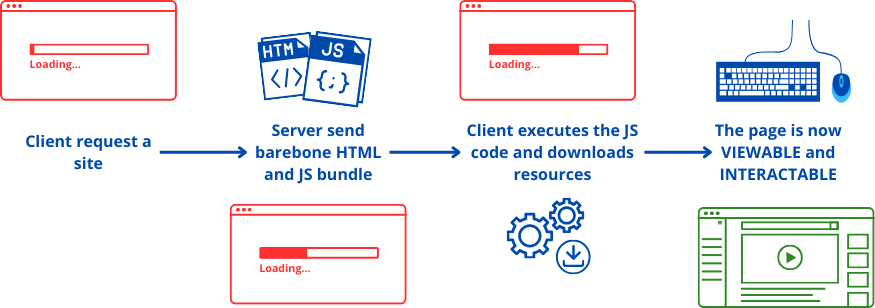
\includegraphics[width=0.7\textwidth]{architectures/CSR.png}
    \caption{Processo di rendering lato client (CSR)}
    \label{fig:CSR}
\end{figure}

Il CSR, o rendering lato client, è una tecnica in cui il processo di rendering avviene appunto sul client, in genere nel browser Web dell'utente.\\
In sintesi, il server invia un documento HTML minimo insieme ai file JavaScript al client. Il browser quindi esegue il
codice JavaScript, il quale è responsabile del recupero dei dati dalle eventuali API, della generazione e della
manipolazione del Document Object Model (DOM) per aggiornare l'interfaccia utente. \\
Nella figura \ref{fig:CSR} è mostrato il processo di rendering lato client.

\color{red}
\paragraph{Esempio di CSR:}
Consideriamo il feed di un social media che deve mostrare un elenco di post. Con CSR, l'HTML e il JavaScript iniziali
vengono inviati al client. Il codice JavaScript, eseguito sul client, recupera quindi i dati del post da un'API e li
visualizza dinamicamente nel browser dell'utente. Mentre l'utente scorre, altri post possono essere recuperati in modo
asincrono, consentendo una paginazione fluida senza dover ricaricare l'intera pagina.
\color{black}